\section{Descriptive Statistics}

\begin{paracol}{2}

\begin{center}
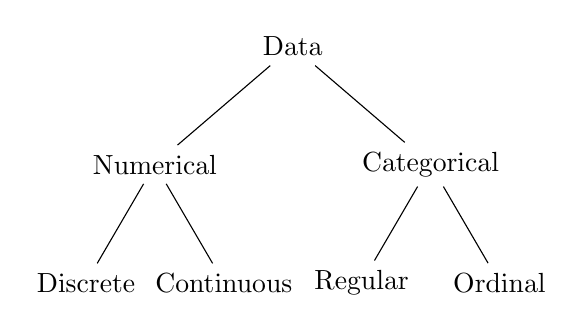
\begin{tikzpicture}[level distance=1.5cm,
  level 1/.style={sibling distance=3.5cm},
  level 2/.style={sibling distance=1.75cm}]
  \node {Data}
    child {node {Numerical}
      child {node {Discrete}}
      child {node {Continuous}}
    }
    child {node {Categorical}
      child {node {Regular}}
      child {node {Ordinal}}
    };
\end{tikzpicture}
\end{center}

\switchcolumn

Observational data come from observing the world as it is.

Experimental data are generated by designing an experiment to test the effect of some explanatory variable, e.g. giving a treatment to the treatment group while not giving it to the control group (/only pretending to treat them).

A summary \textbf{statistic} is a number summarising the data, e.g. the mean, median (middle value), mode (most common value), variance.

\end{paracol}

Imagine we take a sample of $n$ observations from a population and calculate a sample statistic. Now imagine we take another $n$ observations and another $n$ observations, etc., and each time we calculate the sample statistic. We can then plot the distribution of the sampling statistic - this is a \textbf{sampling distribution}. By the CLT, for a large number of successive random samples (big $n$), the distribution of sample means calculated for each sample will become approximately normally distributed.

If you take a lot of sample means from the same population, you may get a different result each time and perhaps none of the sample means would exactly equal the true population mean. Therefore, we need to specify a \textbf{margin of error} - a confidence interval. Point estimates vary from sample to sample, and we quantify this variability with what is called the standard error - the standard deviation of the sampling distribution:

\vspace{-20pt}

$$SE = \sqrt{\text{Var}(\bar{X}) = \sqrt{\frac{\sigma^2}{n}}}$$

\vspace{-10pt}

Confidence interval: point estimate $\pm z^* \times SE$, where $z^* \times SE$ is the margin of error.

\subsection{Connection with Probability Theory}

\begin{tikzpicture}
\node [rounded-box] (box){\begin{minipage}{0.975\textwidth}
    Consider a dataset consisting of $n$ repeated measurements. Then the observations can be modelled by a \textbf{statistical model} as realisations of random variables $X_1, X_2, \dots, X_n$ such that they are \textbf{i.i.d.} (independent and identically distributed): \\

    \begin{enumerate}
        \item $X_1, X_2, \dots, X_n$ have the same probability distribution.
        \item $X_1, X_2, \dots, X_n$ are independent.
    \end{enumerate}
\end{minipage}};
\node[rounded-box-title, left=10pt] at (box.north east) {Definition};
\end{tikzpicture}

\vspace{10pt}

\begin{center}
\begin{tabular}{c|c}
    \textbf{Dataset with observations} $x_1, \dots, x_n$ & \textbf{Model with random variables} $X_1, \dots, X_n \sim f$ \\[0.25cm]
    \hline \\[0.125cm]
    Sample mean $\bar{x}_n = \frac{1}{n} \sum_{i=1}^n x_i$ & Expectation $E[X_i]$ \\[0.25cm]
    Sample median $m = \text{median}(x_1, \dots, x_n)$ & 50-th percentile $q_{0.5} = F^{-1}(\frac{1}{2})$ \\[0.25cm]
    Sample variance $s_n^2 = \frac{1}{n-1} \sum_{i=1}^n (x_i - \bar{x}_n)^2$ & Variance $\text{Var}(X_i)$ \\[0.25cm]
    Sample standard deviation $s_n = \sqrt{s_n^2}$ & Standard deviation $\sqrt{\text{Var}(X_i)}$ \\[0.25cm]
    Empirical quantile $q_n(p)$ s.t. $\frac{\# x_i \leq q_n(p)}{n} \leq p$ & $p$-th quantile $q_p = F^{-1}(p)$ \\[0.25cm]
    Sample correlation coefficient $ r_{x, y}$ & Correlation coefficient $\rho(X, Y)$
\end{tabular}
\end{center}

\begin{paracol}{2}

\subsection{Univariate Descriptive Statistics}

\begin{tikzpicture}
\node [rounded-box] (box){\begin{minipage}{0.45\textwidth}
    For a dataset $x_1, x_2, \dots, x_n$, the \textbf{sample variance} is defined as the unbiased estimator

    $$s^2 = \frac{1}{n-1} \sum_{i=1}^n (x_i - \bar{x}_n)^2$$

    The sample standard deviation $s$ is the square root of the variance.
\end{minipage}};
\node[rounded-box-title, left=10pt] at (box.north east) {Definition};
\end{tikzpicture}

A boxplot and a histogram can be used to visualise a univariate dataset with its statistics and distribution.

A normalised \textbf{histogram} has area equal to one. The height of the bar of a given bin is equal to the proportion of data-points divided by the size of the bin.

\switchcolumn

\subsection{Bivariate Descriptive Statistics}

\begin{tikzpicture}
\node [rounded-box] (box){\begin{minipage}{0.45\textwidth}
    For a bivariate dataset $(x_1, y_1), (x_2, y_2), \dots, (x_n, y_n)$, the \textbf{sample correlation coefficient} is

    \vspace{-15pt}

    $$ r_{x, y} = \frac{
    \sum_{i=1}^n (x_i - \bar{x}) (y_i - \bar{y})
    }{\sqrt{
    \sum_{i=1}^n (x_i - \bar{x})^2 \sum_{i=1}^n (y_i - \bar{y})^2
    }} = \frac{s_{xy}}{\sqrt{s_{xx} s_{yy}}}$$

    \vspace{-5pt}

    Properties:

    \begin{enumerate}
        \item $-1 \leq  r_{x, y} \leq 1$.
        \item Thus, the sample correlation coefficient is independent of units of measurement.
    \end{enumerate}
\end{minipage}};
\node[rounded-box-title, left=10pt] at (box.north east) {Definition};
\end{tikzpicture}

A \textbf{scatterplot} can be used to investigate the relationship between two variables.

A \textbf{spurious correlation} is one where there is correlation without causation. A \textbf{latent variable} is an unobserved third variable causing a change in two strongly correlated variables.

\end{paracol}

\begin{verbatim}
data(mtcars)
# View(mtcars)
min(mtcars$wt)
max(mtcars$mpg)
mtcars[mtcars$X == "Duster 360",]
median(c(4, 18, 11, 9, 12, 4, 6, 7))
help(mtcars)
boxplot(mtcars$wt)
round(quantile(mtcars$wt), 3)
round(IQR(mtcars$wt), 3)

data(airquality)
hist(airquality$Temp, breaks=25)
qqnorm(airquality$Temp)
qqline(airquality$Temp, col='red')
hist(airquality$Ozone)
qqnorm(airquality$Ozone)
qqline(airquality$Ozone, col='red')
qqplot(qexp(ppoints(airquality$Ozone)), airquality$Ozone)
qqline(airquality$Ozone, distribution=qexp, col='blue') # not exponential either

set.seed(0)
x <- rnorm(5, mean=0, sd=1)
x
qqnorm(x)
qqline(x, col='red')
# The points are generated randomly from a normal distribution.
# So, it is extremely unlikely that they lie on a straight line.
# When there are more points, small individual deviations do not matter as much,
# and we will be able to draw an almost straight line through the points.

x <- c(3, 5, 7)
y <- c(8, 4, 6)
plot(x, y, xlim = c(0, 10), ylim = c(0, 10), pch = 16, col = "blue", xlab = "x", ylab = "y")
text(x, y, labels = paste("(", x, ",", y, ")", sep = ""), pos = 3)
correlation_coefficient <- cor(x, y)
correlation_coefficient # -0.5

# install.packages("ggplot2movies")
library(ggplot2movies)
data(movies)
plot(movies$year, movies$votes, xlab = "Year", ylab = "Votes")
round(cor(movies$year, movies$votes), 3)

set.seed(0)
x <- rexp(10, 3)
lambda_hat <- 1 / mean(x) # mean = 1 / lambda
round(lambda_hat, 2)
lambda_hat <- log(2) / median(x) # median = log(2) / lambda
round(lambda_hat, 2)
lambda_hat <- sqrt(1 / var(x)) # var = 1 / lambda^2
round(lambda_hat, 2)
set.seed(0)
x <- rexp(100, 3)
lambda_hat <- 1 / mean(x) # mean = 1 / lambda
round(lambda_hat, 2)
lambda_hat <- log(2) / median(x) # median = log(2) / lambda
round(lambda_hat, 2)
lambda_hat <- sqrt(1 / var(x)) # var = 1 / lambda^2
round(lambda_hat, 2)
# The estimates get better as the number of data points increases.

\end{verbatim}
